\chapter {Quick Reference: Component Details}
%%%%%%%%%%%%%%
\section{Intermediate Frequency Transformer}
\label{IFT}

\begin{figure}[ht]
\centering{ 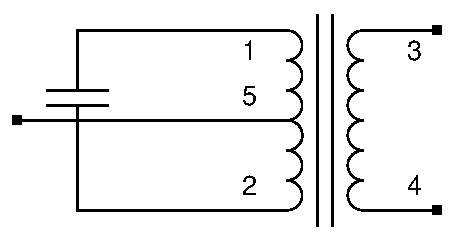
\includegraphics[]{ift.eps}}
\caption {Schematic diagram of intermediate frequency transformer}
\label{iftschem}
\end{figure}


Intermediate Frequency Transformers come as specially designed tuned circuits in groundable metal packages called IF cans. The primary winding has an inducance of $L_{eq}=450\mu H$ and it comes with a shunt capacitor of capacitance $C=270\ pF$. Its resonant frequency is thus $f=\frac{1}{2\pi\sqrt{L_{eq}C}}\approx 455 kHz$.

This frequecy is adjustable by a factor of $\pm 10 \%$ . IFT has a tapped primary winding as shown in the schematic diagram, Figure \ref{iftschem}. 

The ferrite core between primary and secondary windings is tunable with a non-metallic screw driver or tuning tool. It changes the mutual inductance and thus control the Q-factor of the collector circuit of connected transistor\cite{Tomasi}. Its internal details are shown in Figure \ref{ifcan2} and physical consruction is shown in Figure \ref{ifcan1} \cite{IFCAN}. \footnote{Images are taken from: \url{http://retro.co.za/archive/amateur/SM0VPO-ReusingIFCans.pdf}}

\begin{figure}
\centering{ 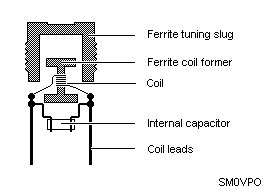
\includegraphics{ifcan2.png}}
\caption {Internal details of IF CAN}

\label{ifcan2}
\end{figure}
\begin{figure}[ht]
\centering{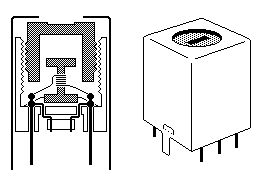
\includegraphics{ifcan1.png}}%[width=\textwidth]
\caption {Physical construction of IF CAN}
\label{ifcan1}
\end{figure}

%%%%%%%%%%%

\section{BJT BF194/195}
\label{BF194/195}
BF194/195 is a high frequency transistor with the following characteristics. \\

Type Designator: BF194/BF195

Material of transistor: Si

Polarity: NPN

Maximum collector power dissipation ($Pc$), W: 0.25

Maximum collector-base voltage |$V_{cb}$|, V: 30

Maximum collector-emitter voltage |$V_{ce}$|, V: 20

Maximum emitter-base voltage |$V_{eb}$|, V: 5

Maximum collector current |$I_{c max}$|, mA: 30

Forward current transfer ratio (hFE), min: 67

%\textcolor{red}{TODO: Pinout diagram to be added}

%\section{OA79 - High frequency diode}
%\textcolor{red}{TODO: Details to be added}
\section{BJT BC107}
\label{BC107}
\noindent Type Designator: BC107

Material of transistor: Si

Polarity: NPN

Maximum collector power dissipation ($P_c$), W: 0.3

Maximum collector-base voltage |$V_{cb}$|, V: 50

Maximum collector-emitter voltage |$V_{ce}$|, V: 45

Maximum emitter-base voltage |$V_{eb}$|, V: 6

Maximum collector current |$I_{cmax}$|, A: 0.1

Forward current transfer ratio ($h_{FE}$), min: 110

Package of BC107 transistor: TO18
%\textcolor{red}{TODO: add schematic diagram and photo of BC107}



\section{CD 4016 - CMOS switching IC}
\label{4016}
The 4016 contains 4 analogue bilateral switches, each with an active-high enable input (A) and two input/outputs (X and Y). When the enable input is asseted (high), the X and Y terminals are connected by a low impedance; this is the on condition. When the enable is low, there is a high impedance path between X and Y, and the switch is off.

The pinout diagram of 4016 switching IC is shown in Figure. \ref{4016pin}\footnote{Image courtesy:\href{http://commons.wikimedia.org/wiki/File\%3A4016\_Pinout.svg}{Inductiveload (Own work) [Public domain]via Wikimedia Commons}}.
\begin{figure}
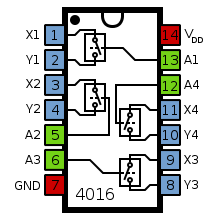
\includegraphics[width=\textwidth, height=7cm]{4016pinout.png}
\caption{Pinout Diagram of 4016 switching IC}
\label{4016pin}
\end{figure} 

\section{AD 633 - Multiplier IC}
\label{AD633}
\paragraph{Multiplier ICs:}
 Analog multipliers are complex arrangements of Opamps and other circuit elements in the form of IC. It can be used for different applications like multiplication, division, squarer, modulator, demodulator, filter etc. There are two inputs $\textbf{X}$ and $\textbf{Y}$ to which the signals to be multiplied are given.
There are two input terminals $\textbf{X}$ and $\textbf{Y}$ to which the signals to be multiplied are given. The output W is the product of instantaneous values of input signals reduced by a scale factor $\textbf{k}$. $\textbf{k}$ is usually less than 1. For practical ICs $\textbf{k}=\frac{1}{10}$.

\begin{equation}
W=kXY
\end{equation}

\begin{figure}[h]
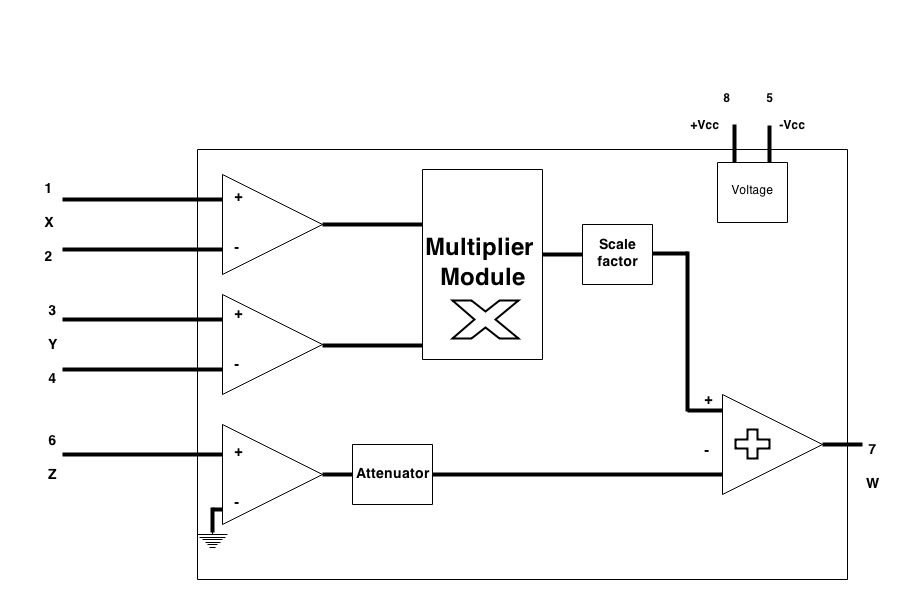
\includegraphics[width=10cm, height=7cm]{ad633.png}
\caption{Functional Block Diagram for AD633 multiplier IC}
\label{ad633}
\end{figure}

\paragraph{AD633} is functionally a complete four quadrant analog multilier IC. The functional block diagram is shown in Fig. \ref{ad633}. This IC uses Gilbert's transconducatnce multiplier module in four quadrants. On chip circuit provides a scale factor of $k=\frac{1}{10}$. If $\textbf{X}$, $\textbf{Y}$ and $\textbf{Z}$ inputs are given we get 
\begin{equation}
W=\frac{XY}{10}+Z
\end{equation}

Here $\textbf{Z}$ is the input to the summing amplifier. If the summing amplifier input is grounded, then output 
\begin{equation}
W=\frac{XY}{10}
\end{equation}

\paragraph{Specifications}as in AD633 data sheet is,

\noindent Dual power supply: $V_{cc}= \pm \ 8V to \pm \ 18V$

\noindent Input impedance > $5 M \Omega$

\noindent Output impedance < $75  \Omega$

\noindent Maximum operating frequency (Bandwidth) = $1 M\Omega$




\section{555 Timer IC}
\label{555}
\begin{figure}[h]
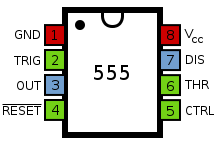
\includegraphics[height=5cm,width=\textwidth]{555_Pinout.png}
\caption{Pin-out diagram of 555 IC}
\end{figure}
The 555 timer IC is an integrated circuit (chip) used in a variety of timer, pulse generation, and oscillator applications. The 555 can be used to provide time delays, as an oscillator, and as a flip-flop element. All these circuit variats are achieved by connecting proper values of resistors and capacitors externally.
The pinout\footnote{Image courtesy:\href{https://commons.wikimedia.org/wiki/\%3A555\_Pinout.svg}{Inductiveload (Own work) [Public domain]via Wikimedia Commons}}. %and internal block diagram\footnote{\url{https://commons.wikimedia.org/wiki/File\%3ANE555_Bloc_Diagram.svg}} 
of 555 timer IC are shown below.
%Its DIP\footnote{\url{https://commons.wikimedia.org/wiki/File\%3ASignetics_NE555N.JPG}} is also shown.


%
%\begin{figure}[h]
%
%
%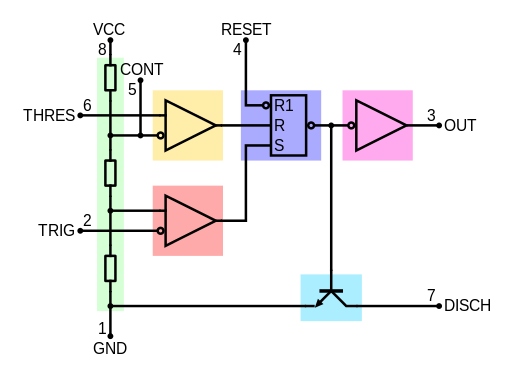
\includegraphics[height=6cm,width=\textwidth]{555blockdiag.png}
%\caption{The internal block diagram of 555 IC}
%
%\end{figure}
\begin{table}
\caption{Pin details of 555 IC}

\label{555pindetails}

\begin{tabular}{|l|l|l|}


\hline
Pin number& Name& Purpose \\
\hline
1&	GND	& Ground reference voltage, low level (0 V)\\
\hline
2&	TRIG	& The OUT pin goes high and a timing interval starts when this input falls below\\& &  1/2 of  CTRL voltage (which is typically 1/3 of VCC, when CTRL is open).\\
\hline

3&OUT	&This output is driven to approximately 1.7 V below +VCC or GND.\\
\hline

4	& RESET &	A timing interval may be reset by driving this input to GND,\\& &  but the timing does not begin again until RESET\\& &  rises above approximately 0.7 volts. Overrides TRIG which overrides THR.\\
\hline

5&	CTRL&	Provides "control" access to the internal voltage divider \\& & (by default, 2/3 VCC).\\ \hline
6&	THR& 	The timing (OUT high) interval ends when the voltage at \\& & THR is greater than that at CTRL (2/3 VCC if CTRL is open).\\ \hline

7&	DIS&	Open collector output which may discharge a capacitor \\& & between intervals. In phase with output.\\ \hline
 
8&	VCC	& Positive supply voltage, which is usually between 3 and 15 V \\& &  depending on the variation.\\ \hline

 

\end{tabular}
\end{table}
The functions of various pins of 555 are shown in Table \ref{555pindetails}. \footnote{\url{https://en.wikipedia.org/wiki/555_timer_IC\#Pins}}

Please refer to \href{https://en.wikipedia.org/wiki/555_timer_IC}{555 Timer IC} for more detailed working of the IC pins when it is configured as multivibrators or oscillators.

%\begin{figure}
%
%
%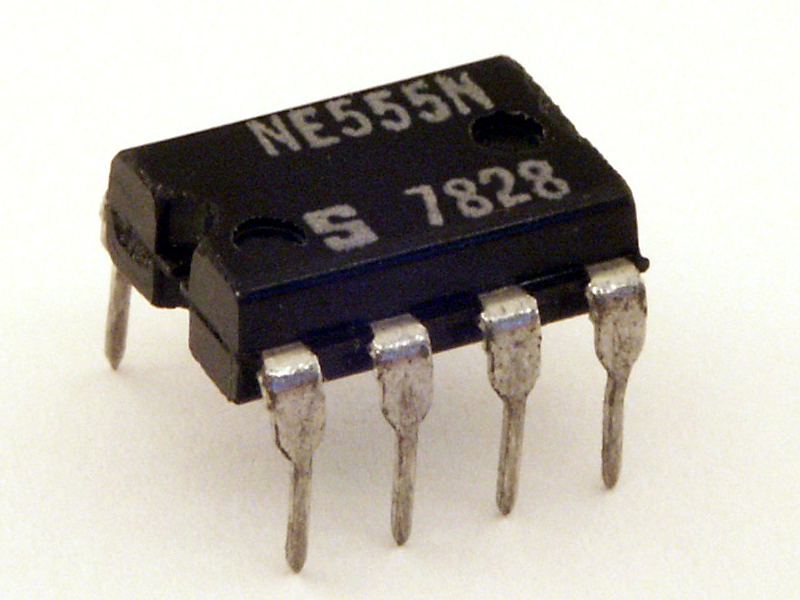
\includegraphics[height=5cm,width=\textwidth]{Signetics_NE555N.jpg}
%\caption{The dual in line package of 555 IC}
%\end{figure}


\section{CD 4046 - PLL IC}
\label{4046}
A phase-locked loop or phase lock loop (PLL) is a control system that generates an output signal from an oscillator which is synchronized in phase and frequency with its input signal. It is an electronic circuit consisting of a voltage controlled variable frequency oscillator(VCO), a phase detector and a lowpass filter. The oscillator generates a periodic signal. The phase detector compares the phase of that signal with the phase of the input periodic signal. Proportional to the phase difference a voltage waveform is generated. It is lowpass filtered to obtain a dc volatge which is proportional to the phase difference. This voltage is fed back to the VCO to control and adjust the oscillator to keep the phases matched. For more details refer \cite{wikipll}. Specifically PLL synchronizes its VCO phase and frequency with the input for a given range of frequencies. The block diagramatic representation of a PLL is shown in Figure. \ref{pll}.

The range of input frequencies($f_i=f_{min}$ to $f_i=f_{max}$) for which the the PLL remains in this locked condition is called lock range of the PLL. If PLL is initially locked and the input fequency $f_i$ becomes less than $f_{min}$ or if $f_i$ exceeds $f_{max}$, PLL becomes unlocked. 

When PLL is unlocked, VCO oscillates at free running frequency or centre frequency, $f_0$. The lock can be re-established if $f_i$ becomes sufficiently close to $f_0$. The range of frequencies around $f_0$(ie, $f_0-f_{cap}$ to $f_0+f_{cap}$) which when applied as input captures a PLL into lock is called capture range of the PLL.

\begin{figure}
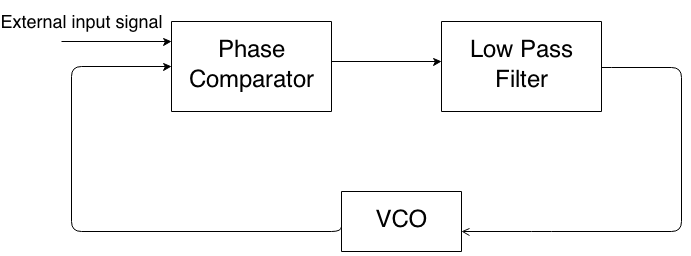
\includegraphics[width=\textwidth]{PLL.png}
\caption{Block diagram of a PLL}
\label{pll}
\end{figure}

\paragraph{}


CD4046 is a PLL IC. It has a linear voltage controlled oscillator(VCO) and two phase comparators($PC_1$ and $PC_2$)-\emph{Any of which can be used for PLL operation}. The periodic signal generated by the VCO is the output signal which is synchronized with the input signal. 

The amplitude of VCO output depends on $V_{cc}$ and its free running frequency is determined by $V_{cc}$ as well as the value of externally connected resistors and capacitors $R_1$, $R_2$ and C. The pinout diagram is shown in the Figure. \ref{pll4046}.

\begin{figure}
\centering{ 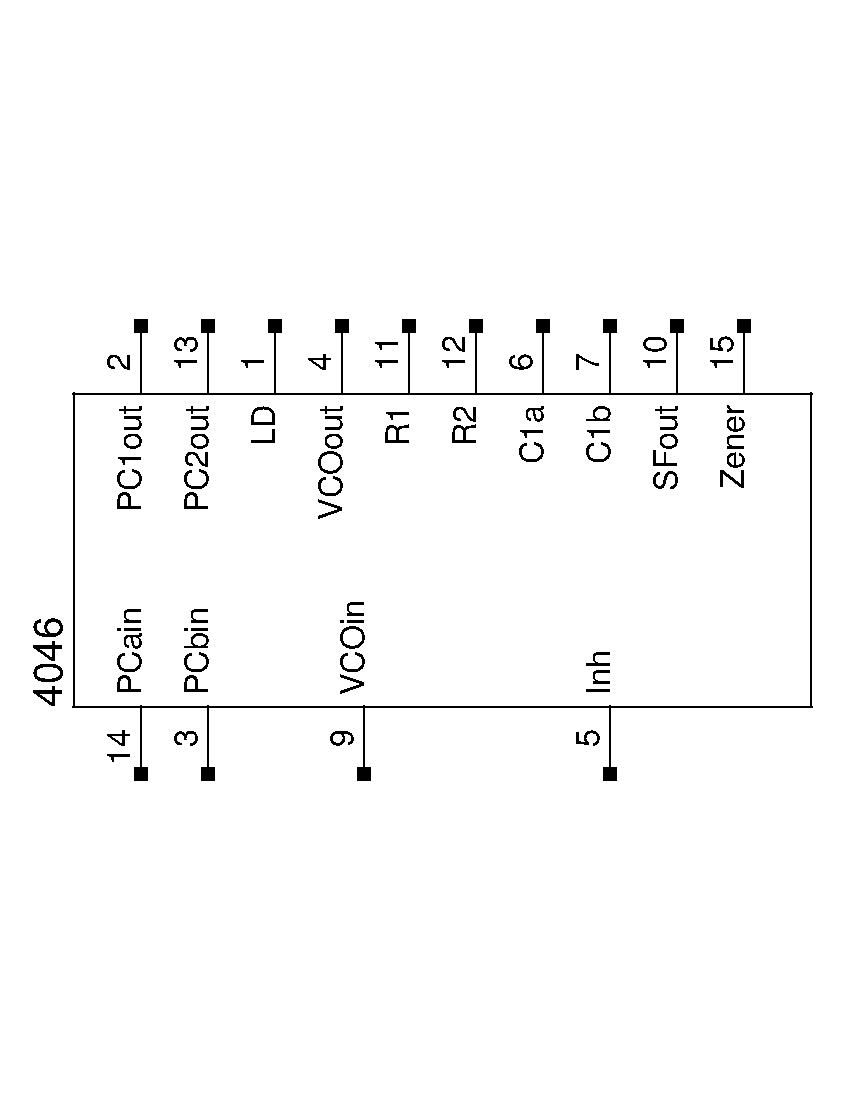
\includegraphics[width=5cm, height=10cm, angle=-90]{4046.png}}%[width=5cm,height=8cm]%
\caption{Pinout diagram of CD4046 PLL IC}
\label{pll4046}
\end{figure}


